\chapter{Laboratory Generation and Lifecycle Management}
\label{chap:laboratory-generation}

The previous chapter described the YAML configuration model and the validation
rules applied before a laboratory is created. At that point the framework has a
validated Python representation of the intended topology, but no Kathar\'a
laboratory has yet been written to disk. This chapter follows the next stage of
the workflow: the transformation of that representation into standard Kathar\'a
artefacts and the management of the resulting laboratory during its operational
lifecycle.

The implementation discussed here is centred on \path{generate_lab.py},
\path{src_gen_lab/gen_lab.py}, and the lifecycle wrappers
\texttt{start.sh}, \texttt{stop.sh}, and \texttt{del\_lab.sh}. The objective is
not to introduce another execution environment on top of Kathar\'a. Instead,
the framework generates the same files that would normally be written by hand:
\texttt{lab.conf}, one startup file for each node, optional per-node resource
directories, and FRRouting configuration files where required. Once those
artefacts have been produced, the laboratory can be started and inspected with
ordinary Kathar\'a commands \cite{kathara_manpage}.

The chapter is deliberately restricted to topology generation and lifecycle
management. It therefore describes how a laboratory is produced, started,
inspected, stopped, and removed, while later experimental procedures are kept
separate from the generation framework itself.

\section{Laboratory Generation Process}
\label{sec:laboratory-generation-process}

The public entry point of the generator is the executable Python script
\path{generate_lab.py}. Its implementation is intentionally minimal: it
imports the \texttt{main()} function from \path{src_gen_lab/gen_lab.py} and
returns its exit status. This separation became more important as generation
grew beyond the first prototype. Keeping argument handling, validation,
FRRouting generation, resource import, and optional monitoring in one root-level
script would have increased coupling and made individual functions harder to
reuse or test. The implementation was therefore organised so that the public
command remains small while the generation logic lives in a dedicated module.
The practical effect is to keep core functions available independently of the
wrapper without turning the project into a monolithic command-line script.

\begin{lstlisting}[language=Python,caption={Command-line wrapper used to start the generator.},label={lst:generator-wrapper}]
#!/usr/bin/env python3
import sys
from src_gen_lab.gen_lab import main

if __name__ == "__main__":
    sys.exit(main())
\end{lstlisting}

The complete generation workflow is shown conceptually in
Figure~\ref{fig:generation-pipeline}. The first three steps correspond to the
loading and validation process described in Chapter~\ref{chap:configuration-validation}.
Only after both structural and semantic validation have succeeded does the
framework prepare the output directory and begin writing Kathar\'a files.

\begin{figure}[htbp]
\centering
\begin{tikzpicture}[
    node distance=8mm,
    box/.style={draw, rounded corners, align=center, minimum width=7.5cm, minimum height=8mm},
    arrow/.style={-{Latex[length=2mm]}, thick}
]
\node[box] (yaml) {YAML configuration};
\node[box, below=of yaml] (load) {Path resolution and safe loading};
\node[box, below=of load] (validate) {Structural and semantic validation};
\node[box, below=of validate] (prepare) {Output-directory preparation};
\node[box, below=of prepare] (labconf) {Generation of \texttt{lab.conf}};
\node[box, below=of labconf] (startup) {Generation of node startup files};
\node[box, below=of startup] (frr) {Generation of FRRouting files where required};
\node[box, below=of frr] (resources) {Optional import of node resources and Wireshark integration};
\node[box, below=of resources] (output) {Executable Kathar\'a laboratory};

\draw[arrow] (yaml) -- (load);
\draw[arrow] (load) -- (validate);
\draw[arrow] (validate) -- (prepare);
\draw[arrow] (prepare) -- (labconf);
\draw[arrow] (labconf) -- (startup);
\draw[arrow] (startup) -- (frr);
\draw[arrow] (frr) -- (resources);
\draw[arrow] (resources) -- (output);
\end{tikzpicture}
\caption{Generation pipeline from a YAML source to an executable Kathar\'a laboratory.}
\label{fig:generation-pipeline}
\end{figure}

The command-line interface exposes the options that control this process.
Table~\ref{tab:generation-cli} summarises the options relevant to general
laboratory generation. The positional \texttt{lab} argument accepts either a
configuration name or an explicit YAML path. The default search directory is
\texttt{configs/}, while generated laboratories are written under
\texttt{labs/} unless a different output path is selected.

\begin{table}[htbp]
\centering
\small
\begin{tabular}{p{0.27\textwidth}p{0.61\textwidth}}
\toprule
\textbf{Argument or option} & \textbf{Purpose} \\
\midrule
\texttt{lab} & Selects the YAML configuration by name or explicit path. \\
\cliopt{config-dir DIR} & Changes the directory searched when \texttt{lab} is not an explicit path. The default is \texttt{configs/}. \\
\cliopt{output-dir DIR}, \texttt{-o DIR} & Changes the parent directory in which the generated laboratory is created. The default is \texttt{labs/}. \\
\cliopt{validate-only} & Executes loading and validation without creating or modifying laboratory files. \\
\cliopt{clean} & Removes an existing laboratory directory and recreates it from the current configuration. \\
\cliopt{force} & Allows generated files to be written inside an already existing laboratory directory. \\
\cliopt{import-dirs} & Copies directories located next to the YAML file when their names match declared nodes. \\
\cliopt{wireshark MODE} & Controls interactive Wireshark integration. The accepted modes are \texttt{ask}, \texttt{enabled}, and \texttt{disabled}. \\
\cliopt{wireshark-networks LIST} & Explicitly selects one or more collision domains to which the generated Wireshark node is attached. \\
\bottomrule
\end{tabular}
\caption{General command-line options used during laboratory generation.}
\label{tab:generation-cli}
\end{table}

A minimal laboratory can therefore be generated using only its configuration
name:

\begin{lstlisting}[language=bash,caption={Generating the minimal client-router-server laboratory.},label={lst:generate-basic}]
python3 generate_lab.py client-router-server
\end{lstlisting}

The same input can be validated without writing any output:

\begin{lstlisting}[language=bash,caption={Validation without generation.},label={lst:generate-validate-only}]
python3 generate_lab.py client-router-server --validate-only
\end{lstlisting}

For a topology that should be rebuilt from a clean state, the usual invocation
is:

\begin{lstlisting}[language=bash,caption={Clean regeneration of a laboratory.},label={lst:generate-clean}]
python3 generate_lab.py multi-area --clean
\end{lstlisting}

The output-directory policy is implemented by \texttt{prepare\_lab\_directory()}.
If the target directory does not exist, it is created. If it exists and
\cliopt{clean} has been requested, the complete directory is removed with
\texttt{shutil.rmtree()} and then recreated. If it exists and neither
\cliopt{clean} nor \cliopt{force} has been supplied, generation stops with
a \texttt{FileExistsError}. With \cliopt{force}, the existing directory is
kept and individual generated files are overwritten as they are produced.

This distinction is important for reproducibility. A clean generation ensures
that every file in the resulting directory derives from the current source
configuration or from resources explicitly copied during the same run. A forced
generation is convenient while developing a topology, because it avoids
removing the directory first, but files that are no longer generated may remain
from an earlier version. For this reason, \cliopt{clean} provides the clearer
operation when the objective is to reconstruct a laboratory from its source.

Normal execution validates the configuration twice at different abstraction
boundaries. The \texttt{main()} function first resolves and validates the input
before any output operation is attempted. The lower-level
\texttt{generate\_lab()} function then loads the selected YAML again and repeats
structural and semantic validation before writing files. Although this produces
some duplicated work, it gives the generation function an independent safety
property: it does not assume that every future caller has already performed
validation correctly. This was an intentional development trade-off: a clear
and defensive module boundary was initially preferred to removing a small
amount of repeated work. The stress tests in
Chapter~\ref{chap:robustness-security-scalability} later made the cost of this
choice measurable and motivated a possible refactoring in which an already
validated in-memory representation can be passed to an internal generation
function.

Once validation has succeeded, \texttt{generate\_lab()} derives the laboratory
name from \texttt{lab\_name}, prepares the output directory, writes
\texttt{lab.conf}, optionally imports node directories, creates every startup
file, creates FRRouting files for FRR-capable devices, removes obsolete
Wireshark helper scripts, and finally returns the generated path and a summary
of optional components. The command-line layer then prints the exact commands
that can be used to start and stop the laboratory. A successful generation is
therefore not only a file-production step but also the transition from the
framework-specific YAML source to a standard Kathar\'a project directory.

\section{Generated Laboratory Structure and Resources}
\label{sec:generated-laboratory-structure}

The most direct way to understand the generator is to examine the artefacts it
creates. Consider the \texttt{client-router-server.yml} configuration contained
in the repository. It defines a client on \texttt{lan1}, a router connected to
both \texttt{lan1} and \texttt{dmz}, and a server on the DMZ. The relevant
source structure is shown in Listing~\ref{lst:chapter4-yaml-example}.

\begin{lstlisting}[caption={Extract from the client-router-server YAML configuration.},label={lst:chapter4-yaml-example}]
lab_name: client-router-server

nodes:
  client:
    type: host
    interfaces:
      - network: lan1
        ip: 10.0.1.10/24
    default_gateway: 10.0.1.1

  router:
    type: router
    interfaces:
      - network: lan1
        ip: 10.0.1.1/24
      - network: dmz
        ip: 10.0.2.1/24

  server:
    type: host
    interfaces:
      - network: dmz
        ip: 10.0.2.10/24
    default_gateway: 10.0.2.1
\end{lstlisting}

With Wireshark disabled and no node directories imported, generation produces
the structure in Listing~\ref{lst:generated-basic-tree}. The router directory
exists because router nodes are considered FRR-capable and therefore receive
an FRRouting directory even when no dynamic protocol has been requested.

\begin{lstlisting}[caption={Generated structure of the minimal routed laboratory.},label={lst:generated-basic-tree}]
labs/client-router-server/
|-- lab.conf
|-- client.startup
|-- router.startup
|-- server.startup
`-- router/
    `-- etc/
        `-- frr/
            |-- daemons
            |-- frr.conf
            `-- vtysh.conf
\end{lstlisting}

The first output file is \texttt{lab.conf}. Its purpose is to describe the
Kathar\'a topology rather than the IP configuration of individual nodes. The
function \path{generate_lab_conf()} begins with metadata and then iterates
through the nodes in the validated configuration. Every interface entry is
translated into a Kathar\'a attachment of the form
\texttt{node[index]="collision-domain"}. The index is the position of the
interface in the YAML list. Consequently, the first interface becomes
\texttt{eth0}, the second becomes \texttt{eth1}, and the same ordering is
subsequently used when the startup file assigns IP addresses.

For the configuration in Listing~\ref{lst:chapter4-yaml-example}, the generated
node definitions are:

\begin{lstlisting}[caption={Topology entries generated in lab.conf.},label={lst:generated-labconf}]
client[0]="lan1"
client[image]="kathara/base"

router[0]="lan1"
router[1]="dmz"
router[image]="kathara/frr"

server[0]="dmz"
server[image]="kathara/base"
\end{lstlisting}

The absence of IP addresses from \texttt{lab.conf} is intentional. The file
answers the question of which node interfaces are attached to which collision
domains. Layer-3 configuration is kept in the corresponding startup files. This
separation follows the normal Kathar\'a laboratory model and is preserved by
the generator rather than hidden behind a new proprietary representation.

The generator also writes the laboratory metadata at the beginning of
\texttt{lab.conf}. Values can be provided through the top-level
\texttt{metadata} mapping. Within that mapping, the \texttt{description}
field takes precedence over the simpler top-level description; default values
are used when individual metadata fields are absent. The output contains fields
for the laboratory description, version, author, email address, and web
reference. These fields do not influence
forwarding, but they make the generated laboratory easier to identify and
trace independently from its YAML source.

Image selection is performed by \texttt{get\_node\_image()}. An explicit
\texttt{image} field always has priority. Without an override, an ordinary host
uses \texttt{kathara/base}. Nodes whose type is \texttt{router},
\texttt{switch}, or \texttt{firewall} use \texttt{kathara/frr}. A host can also
become FRR-capable when it contains an active \texttt{frr} section. This policy
provides useful defaults while still allowing the YAML configuration to select
a different image when the node requires additional software.

After \texttt{lab.conf}, the generator creates one \texttt{.startup} file
for every node. The startup-generation function processes the same ordered
interface list used by \texttt{lab.conf}. For every interface that
contains an IP address, it generates an \texttt{ip address add} command and
associates the address with \texttt{ethN}. For example, the client in the
minimal topology produces:

\begin{lstlisting}[language=bash,caption={Generated startup file for the client node.},label={lst:client-startup}]
ip address add 10.0.1.10/24 dev eth0

ip route add default via 10.0.1.1
\end{lstlisting}

The router produces:

\begin{lstlisting}[language=bash,caption={Generated startup file for the router node.},label={lst:router-startup}]
ip address add 10.0.1.1/24 dev eth0
ip address add 10.0.2.1/24 dev eth1

systemctl start frr
\end{lstlisting}

The generator does not emit explicit \texttt{ip link set ethN up} commands.
Kathar\'a creates the interfaces as part of the node environment, while the
startup file assigns addresses and routing state. This detail is relevant when
describing the implementation because the generated file should be documented
as it actually exists rather than as a generic Linux-network configuration
procedure.

Default gateways and static routes are translated directly into Linux route
commands. A YAML route such as

\begin{lstlisting}[caption={Static route represented in YAML.},label={lst:static-route-yaml}]
routes:
  - to: 192.168.20.0/24
    via: 10.0.12.2
\end{lstlisting}

becomes:

\begin{lstlisting}[language=bash,caption={Command generated from a static route.},label={lst:static-route-generated}]
ip route add 192.168.20.0/24 via 10.0.12.2
\end{lstlisting}

The \texttt{commands} list is handled differently. Its entries are not
translated into a framework-defined representation; they are appended to the
startup file as literal strings after the automatically generated network and
FRR commands. The model therefore has a clear boundary. Common operations such
as address assignment, gateways, routes, and routing-daemon startup are
produced automatically, while node-specific behaviour can still be expressed
through arbitrary startup commands when needed.

Table~\ref{tab:yaml-to-generated} summarises the relationship between the main
configuration operations introduced in Chapter~\ref{chap:configuration-validation}
and their generated output.

\begin{table}[htbp]
\centering
\small
\begin{tabular}{p{0.28\textwidth}p{0.29\textwidth}p{0.31\textwidth}}
\toprule
\textbf{YAML information} & \textbf{Generated artefact} & \textbf{Effect} \\
\midrule
Node name & \texttt{lab.conf}, startup filename, optional node directory & Establishes the node identifier used throughout the laboratory. \\
\texttt{interfaces[].network} & \texttt{lab.conf} & Connects \texttt{ethN} to a Kathar\'a collision domain. \\
\texttt{interfaces[].ip} & \texttt{<node>.startup} & Adds the configured address to the corresponding interface. \\
\texttt{default\_gateway} & \texttt{<node>.startup} & Adds the node's default route. \\
\texttt{routes} & \texttt{<node>.startup} & Adds explicit static routes. \\
\texttt{commands} & \texttt{<node>.startup} & Appends user-provided shell commands literally. \\
\texttt{image} or inferred node role & \texttt{lab.conf} & Selects the container image. \\
\texttt{frr} & \texttt{<node>/etc/frr/*} and startup file & Creates FRRouting files and starts the FRR service. \\
\bottomrule
\end{tabular}
\caption{Relationship between source configuration fields and generated Kathar\'a artefacts.}
\label{tab:yaml-to-generated}
\end{table}

FRRouting generation is integrated into the same output process. The helper
\texttt{is\_frr\_device()} determines whether a node receives FRR files. Device
types \texttt{router}, \texttt{switch}, and \texttt{firewall} are always
considered FRR-capable. For a host, the presence of an enabled \texttt{frr}
section is sufficient. This behaviour means that a router without an explicitly
selected dynamic protocol still receives a minimal FRR configuration and its
startup file still runs \texttt{systemctl start frr}.

For each FRR-capable node, \texttt{write\_frr\_files()} creates
\texttt{etc/frr/} under the node directory and writes three files:
\texttt{daemons}, \texttt{frr.conf}, and \texttt{vtysh.conf}, following the
configuration model provided by FRRouting \cite{frr_user_guide}. The daemon file
always enables Zebra and activates the protocol daemons inferred from the YAML.
For a single OSPF router, the relevant part is similar to:

\begin{lstlisting}[caption={Relevant entries in an automatically generated FRR daemons file.},label={lst:frr-daemons}]
zebra=yes
bgpd=no
ospfd=yes
ripd=no
ospf6d=no
ripngd=no
...
vtysh_enable=yes
\end{lstlisting}

The \texttt{frr.conf} file is generated from protocol-specific fields. The
\texttt{multi-area.yml} configuration, for example, declares router \texttt{r1}
with three addressed interfaces and associates its LAN with area 10 and its two
transit links with area 0. The generated configuration is:

\begin{lstlisting}[caption={FRRouting configuration generated for r1 in the multi-area laboratory.},label={lst:generated-ospf-conf}]
frr defaults traditional
hostname r1
service integrated-vtysh-config
!
router ospf
 ospf router-id 1.1.1.1
 network 10.10.1.0/24 area 10
 network 10.0.12.0/30 area 0
 network 10.0.13.0/30 area 0
!
line vty
!
\end{lstlisting}

This example illustrates an important property of the generator: the user
assigns an address and an OSPF area to the interface, while the framework
derives the corresponding network prefix before writing the FRR
\texttt{network} command; the protocol semantics follow OSPFv2 as specified in
RFC~2328 \cite{rfc2328}. The same source information therefore drives both
Linux interface configuration and routing-protocol configuration, reducing
manual duplication between files.

RIP follows the same principle. The generator writes a \texttt{router rip}
section, selects the requested version, disables automatic summarisation by
default, and lists the networks associated with RIP. For BGP, the generator
writes the autonomous-system number, optional router ID, neighbour statements,
advertised prefixes, and redistribution rules where configured
\cite{rfc4271}. A typical
fragment produced from \texttt{multi\_AS.yml} is structurally equivalent to:

\begin{lstlisting}[caption={Example of automatically generated BGP configuration.},label={lst:generated-bgp-conf}]
router bgp 65001
 bgp router-id 1.1.1.1
 no bgp ebgp-requires-policy
 no bgp network import-check
 neighbor 10.0.12.2 remote-as 65002
 neighbor 10.0.13.2 remote-as 65003
 network 10.10.1.0/24
\end{lstlisting}

The two \texttt{no bgp} commands are generated when the corresponding YAML
options retain their default false value. In particular,
\texttt{ebgp-requires-policy} reflects the external-BGP policy behaviour
standardised by RFC~8212 \cite{rfc8212}. They make the behaviour appropriate
for the small controlled laboratories used by the framework: eBGP announcements
are not blocked by the default policy requirement, and a configured
\texttt{network} statement is not suppressed only because the exact route is
absent from the local routing information base at configuration time. These
settings are generation choices for the project environment rather than a
replacement for policy configuration in operational networks.

The generator also supports protocol redistribution and multiple routing
protocols on the same node. Protocol discovery accepts the compact
\texttt{frr.protocol} field, a \texttt{protocols} collection, nested
\texttt{ospf}, \texttt{rip}, and \texttt{bgp} mappings, or direct daemon
markers. This backwards-compatible parsing allows the more structured example
configurations to coexist with simpler earlier files.

A complete \texttt{frr.config} block acts as an escape mechanism: when present,
its content is written directly to \texttt{frr.conf} instead of constructing
the protocol configuration automatically. It is important to distinguish this
from daemon activation. The contents of \texttt{frr.conf} may be supplied
manually, but \texttt{daemons} is still generated from the protocol or daemon
information that the framework can identify. A manual configuration that uses
a protocol daemon should therefore also declare enough information for that
daemon to be enabled. This is one of the points where flexibility transfers
more responsibility to the configuration author.

The third FRR file, \texttt{vtysh.conf}, contains
\texttt{service integrated-vtysh-config}. Together with
\texttt{vtysh\_enable=yes} in the daemon file, it allows the generated router to
be inspected through the standard \texttt{vtysh} interface after the
laboratory starts.

Beyond generated network files, the framework can import arbitrary resources
associated with a node. The option \cliopt{import-dirs} activates
\texttt{copy\_node\_directories()}. The source directory is the directory that
contains the selected YAML file, not necessarily the repository's global
\texttt{configs/} directory. For each declared node, the function checks for a
sibling directory with exactly the same name. If it exists, that directory is
copied recursively into the generated laboratory.

The mapping is therefore:

\begin{lstlisting}[caption={Mapping used when node-specific resources are imported.},label={lst:resource-import-map}]
<directory containing YAML>/<node-name>/ 
                    |
                    |
<output-dir>/<lab-name>/<node-name>/
\end{lstlisting}

For a configuration stored in \texttt{configs/example.yml}, a directory
\texttt{configs/server/} is copied to
\texttt{labs/example/server/}. Kathar\'a exposes the files stored in the node
directory through the node's \texttt{/hostlab/} path. A startup command can
therefore execute an imported script without embedding that script into the
YAML configuration itself. This separation is useful because the YAML remains
focused on topology and startup declarations, while application code, data
files, or node-specific configuration can remain ordinary files.

The import process deliberately ignores \texttt{\_\_pycache\_\_}, compiled
\texttt{.pyc} files, \texttt{.git}, and \texttt{.DS\_Store}. The semantic
validation described in the previous chapter also reports visible sibling
directories that do not correspond to nodes when directory import is enabled.
The generator itself simply skips node names for which no source directory
exists. Resource import is therefore optional and non-invasive: a topology can
be generated with only the files derived from YAML, or enriched with external
per-node resources when required.

Wireshark integration is another optional extension of the generated
\texttt{lab.conf}; Wireshark provides the packet-capture and protocol-analysis
capabilities used by this observation node \cite{wireshark_user_guide}. The
feature was introduced as runtime debugging became more important during
development. Inspecting a generated startup file shows what the framework
intends to configure, but it does not show whether packets actually traverse
the expected collision domain or where communication stops. Packet capture was
therefore kept as an optional diagnostic layer rather than made part of every
functional topology. The implementation first reconstructs the set of collision
domains by scanning all node interfaces. Each domain is associated with the
nodes, interface indices, and optional addresses attached to it. This makes it
possible to present a meaningful selection such as
\texttt{lan\_a | r1:eth0(...), pc\_a:eth0(...)} rather than only a list of
internal names.

A capture point can be selected explicitly from the command line:

\begin{lstlisting}[language=bash,caption={Generating a laboratory with Wireshark attached to two collision domains.},label={lst:wireshark-cli}]
python3 generate_lab.py multi-area --clean \
    --wireshark-networks lan_a,r1_r2
\end{lstlisting}

The parser also accepts \texttt{all}, numeric indexes in interactive mode, or
the form \texttt{node:r1}, which expands to every collision domain attached to
the selected node. A top-level \texttt{wireshark} mapping in the YAML can also
provide an enabled flag and one or more networks. Explicit command-line network
selection takes precedence over interactive selection.

Wireshark is represented as a normal Kathar\'a node added directly to
\texttt{lab.conf}. For a capture on \texttt{lan1}, the generated block is:

\begin{lstlisting}[caption={Wireshark node generated in lab.conf.},label={lst:wireshark-labconf}]
# Wireshark real-time packet capture
wireshark[0]="lan1"
wireshark[bridged]=true
wireshark[port]="3000:3000/tcp"
wireshark[image]="lscr.io/linuxserver/wireshark"
wireshark[num_terms]=0
\end{lstlisting}

Connecting Wireshark to collision domains in \texttt{lab.conf} is preferable
to attaching an external capture process after startup because the observation
point becomes part of the generated topology itself. One Wireshark node may be
attached to several selected domains. When generated in this form, the browser
interface is published on TCP port 3000. The generator also removes the legacy
\texttt{start\_wireshark.sh}, \texttt{sniff.sh}, and
\texttt{stop\_wireshark.sh} files if they still exist in the laboratory
directory, because they are unnecessary once the capture node is defined
directly in \texttt{lab.conf}.


% Conditional runtime evidence requested during thesis review.  The project
% compiles without the image; adding images/wireshark_capture.png enables the
% figure and the accompanying text automatically.
\IfFileExists{images/wireshark_capture.png}{%
\begin{figure}[htbp]
\centering
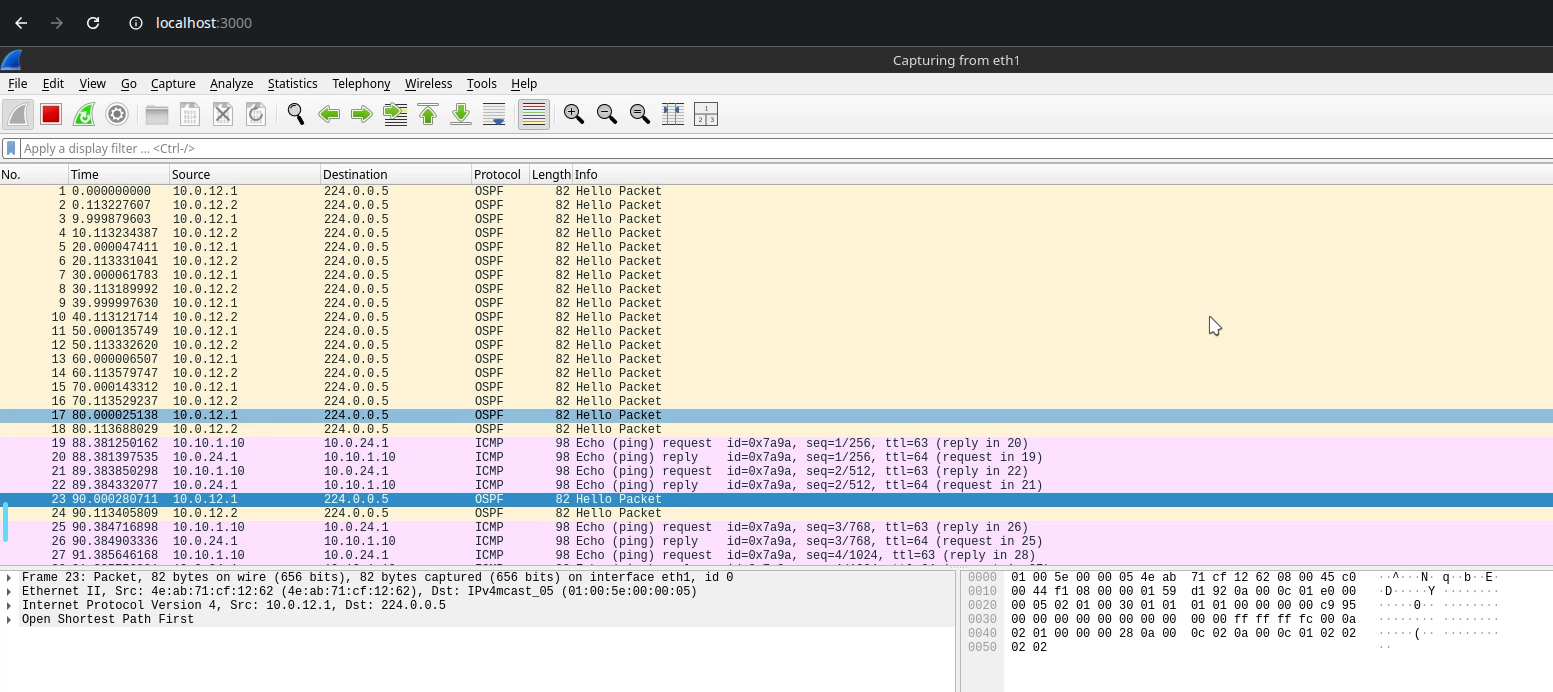
\includegraphics[width=0.92\textwidth,height=0.28\textheight,keepaspectratio]{images/wireshark_capture.png}
\caption{Runtime Wireshark capture on the \texttt{r1\_r2} collision domain of the generated multi-area laboratory.}
\label{fig:wireshark-runtime-capture}
\end{figure}

Figure~\ref{fig:wireshark-runtime-capture} provides a runtime check of the
monitoring integration. The generated Wireshark node is attached to the
selected collision domain and observes packets exchanged by the emulated nodes
without changing their functional roles. This complements inspection of
\texttt{lab.conf}: the generated file proves that the observation node was
configured, while the capture demonstrates that traffic on the selected
Kathar\'a segment is actually visible to it during execution.
}{}

The output of the generation stage is therefore a conventional Kathar\'a
laboratory enriched only by files that Kathar\'a already knows how to consume.
The framework's YAML format is used before generation; it is not required by
Kathar\'a at runtime. This design is significant because a generated laboratory
can be opened, inspected, and started with standard Kathar\'a tools even if the
generator is not invoked again.

\section{Laboratory Execution and Lifecycle Management}
\label{sec:laboratory-lifecycle}

Once generation is complete, the operational workflow returns to ordinary
Kathar\'a commands. The repository provides shell wrappers for the most common
lifecycle operations. Their purpose is intentionally limited: they perform
basic argument and directory checks, change into the selected laboratory, and
invoke the corresponding Kathar\'a command. Generation and runtime management
were deliberately not merged into one long-running Python process, because the
produced laboratory should remain usable even after the generator has exited.
The wrappers reduce repetitive shell navigation while keeping the underlying
Kathar\'a operation visible to the user.

Figure~\ref{fig:lifecycle-loop} presents the intended lifecycle. The YAML file
remains the source configuration. It is validated and generated into a
laboratory directory, which can then be started and inspected. When a persistent
change is required, the change is applied to the YAML source or to a node
resource directory and the laboratory is regenerated rather than relying on a
manual edit to derived output.

\begin{figure}[htbp]
\centering
\begin{tikzpicture}[
    node distance=12mm and 12mm,
    state/.style={draw, rounded corners, align=center, minimum width=2.6cm, minimum height=9mm, font=\small},
    arrow/.style={-{Latex[length=2mm]}, thick}
]
\node[state] (config) {Configure\\YAML source};
\node[state, right=of config] (validate) {Validate};
\node[state, right=of validate] (generate) {Generate\\laboratory};
\node[state, below=of generate] (start) {Start};
\node[state, left=of start] (inspect) {Inspect and\\verify};
\node[state, left=of inspect] (stop) {Stop};

\draw[arrow] (config) -- (validate);
\draw[arrow] (validate) -- (generate);
\draw[arrow] (generate) -- (start);
\draw[arrow] (start) -- (inspect);
\draw[arrow] (inspect) -- (stop);
\draw[arrow] (stop) -- node[pos=0.35,left,align=center]{modify source\\and regenerate}(config);
\end{tikzpicture}
\caption{Operational lifecycle of a generated laboratory.}
\label{fig:lifecycle-loop}
\end{figure}

A laboratory can be started with the wrapper by passing its generated path:

\begin{lstlisting}[language=bash,caption={Starting a generated laboratory.},label={lst:start-lab}]
./start.sh labs/client-router-server
\end{lstlisting}

The script requires at least one argument, derives the display name with
\texttt{basename}, verifies that the supplied directory exists, changes into
that directory, and executes:

\begin{lstlisting}[language=bash,caption={Kathar\'a command executed by start.sh.},label={lst:kathara-lstart}]
kathara lstart
\end{lstlisting}

Starting from the laboratory directory matters because Kathar\'a reads the
local \texttt{lab.conf} and the associated node files. During startup, the
collision-domain definitions in \texttt{lab.conf} determine the emulated links,
container images determine the node environments, and the \texttt{.startup}
files apply addresses, routes, FRRouting startup, and user commands. FRR-capable
nodes also find their configuration under their local
\texttt{/etc/frr/}-equivalent hostlab structure according to the standard
Kathar\'a file-mapping mechanism.

The wrapper is not required. The generator explicitly prints the equivalent
manual procedure after a successful run:

\begin{lstlisting}[language=bash,caption={Starting a laboratory without the wrapper.},label={lst:start-manual}]
cd labs/client-router-server
kathara lstart
\end{lstlisting}

Keeping both forms available is useful. The wrapper makes the common operation
shorter, while the explicit commands make it clear that the generated output is
not tied to the framework's own runtime.

After startup, individual nodes can be accessed through normal Kathar\'a
commands. For example:

\begin{lstlisting}[language=bash,caption={Connecting to a generated router.},label={lst:kathara-connect}]
kathara connect router
\end{lstlisting}

Once inside a node, standard Linux tools provide a first verification of the
generated configuration. \texttt{ip addr} shows whether addresses have been
assigned to the expected interface indices, \texttt{ip route} shows connected,
default, and static routes, and \texttt{ping} can be used for a basic
reachability check. In the minimal client-router-server topology, the client
can verify the path to the server address with:

\begin{lstlisting}[language=bash,caption={Basic reachability check after laboratory startup.},label={lst:basic-ping}]
ping 10.0.2.10
\end{lstlisting}

For FRRouting nodes, \texttt{vtysh} provides the corresponding routing view.
Commands such as \texttt{show ip route}, \texttt{show ip ospf neighbor}, and
\texttt{show ip bgp summary} are useful for verifying that the generated FRR
files have been loaded and that protocol state is developing as expected. These
manual checks are not part of generation itself. They are operational
observations performed after the generated files have been consumed by the
runtime environment.

This distinction is important because successful generation does not imply
immediate runtime convergence. The generator can prove that configured OSPF
networks refer to connected prefixes and that BGP neighbour declarations are
coherent according to the static model, but it cannot guarantee that a routing
protocol has converged at the exact moment the containers start. Runtime state
depends on process startup, neighbour availability, timers, imported resources,
and any user-supplied commands. Generation correctness and runtime behaviour
are therefore related but separate concerns.

The repository provides \texttt{stop.sh} for the inverse lifecycle operation:

\begin{lstlisting}[language=bash,caption={Stopping and cleaning the runtime environment.},label={lst:stop-lab}]
./stop.sh labs/client-router-server
\end{lstlisting}

Like \texttt{start.sh}, the script verifies that the supplied directory exists
and changes into it. It then invokes the standard Kathar\'a cleanup command
\cite{kathara_manpage}:

\begin{lstlisting}[language=bash,caption={Kathar\'a command executed by stop.sh.},label={lst:kathara-lclean}]
kathara lclean
\end{lstlisting}

The word \emph{clean} in this Kathar\'a command should not be confused with the
generator's \cliopt{clean} option. \texttt{kathara lclean} removes the
runtime laboratory created by Kathar\'a, including the containers and associated
runtime networking, while the generated directory on disk remains available.
The generator's \cliopt{clean}, by contrast, operates on the file-system
output before generation: it deletes the selected laboratory directory and
recreates its files from the YAML source.

The difference can be summarised as follows:

\begin{table}[htbp]
\centering
\small
\begin{tabular}{p{0.25\textwidth}p{0.31\textwidth}p{0.30\textwidth}}
\toprule
\textbf{Operation} & \textbf{Generated files} & \textbf{Runtime containers and networks} \\
\midrule
Generation & Created or overwritten & Not started by the generator \\
\texttt{start.sh} / \texttt{kathara lstart} & Preserved & Created and started \\
\texttt{stop.sh} / \texttt{kathara lclean} & Preserved & Removed \\
Generation with \cliopt{clean} & Directory removed and regenerated & Independent of runtime state \\
\texttt{del\_lab.sh} & Selected generated directory removed & Does not replace runtime cleanup \\
\bottomrule
\end{tabular}
\caption{Effects of the main lifecycle operations.}
\label{tab:lifecycle-effects}
\end{table}

When the generated files are no longer required, \texttt{del\_lab.sh} removes
them from disk. It accepts either a path to a laboratory directory or the
literal argument \texttt{all}. For an individual laboratory:

\begin{lstlisting}[language=bash,caption={Deleting one generated laboratory.},label={lst:delete-one-lab}]
./del_lab.sh labs/client-router-server
\end{lstlisting}

and for all generated content under \texttt{labs/}:

\begin{lstlisting}[language=bash,caption={Deleting all generated laboratories.},label={lst:delete-all-labs}]
./del_lab.sh all
\end{lstlisting}

The current implementation performs deletion with \texttt{sudo rm -rf}. When
\texttt{all} is supplied, only the contents of \texttt{./labs/} are removed and
the parent directory itself is preserved. For a specific argument, the script
first checks that the path exists as a directory and then removes that path.
Because this is a destructive file-system operation, the selected path should
be verified before invoking the command. In normal use, runtime cleanup with
\texttt{stop.sh} should be treated separately from removal of generated files.

The explicit path accepted by the lifecycle scripts also allows several
laboratories to coexist under the same output directory. A repository may, for
example, contain:

\begin{lstlisting}[caption={Several generated laboratories coexisting under labs/.},label={lst:multiple-labs}]
labs/
|-- client-router-server/
|-- Test1_multi_area/
|-- multi-AS/
`-- Test_enterprise_multi_as_import_dirs/
\end{lstlisting}

No lifecycle script needs to guess which one is active or intended. This
explicit selection also reflects a development issue that appeared as the
number of example configurations increased: assumptions that were harmless
when only one generated laboratory was present became ambiguous once several
outputs coexisted under \texttt{labs/}. The user therefore selects the
laboratory explicitly:

\begin{lstlisting}[language=bash,caption={Starting one laboratory among several generated environments.},label={lst:start-specific-lab}]
./start.sh labs/multi-AS
\end{lstlisting}

This explicit selection is consistent with the framework's general design: the
tool automates repetitive file creation and common commands, but avoids hidden
choices when more than one valid target exists.

The lifecycle also clarifies which artefact should be considered authoritative.
The YAML configuration is the source description, while the directory under
\texttt{labs/} is derived output. A persistent topology change should therefore
be applied to the YAML source. A persistent node-resource change should be
applied to the resource directory located next to that YAML file. After the
change, the laboratory can be regenerated, preferably with \cliopt{clean}
when a fully reconstructed output is required.

Directly editing \texttt{lab.conf}, a generated startup file, or a generated
FRR file is possible because they are ordinary text files, but such edits are
not part of the reproducible source model. A later clean generation replaces
them. Treating generated files as disposable output reduces configuration drift
between the declarative source and the laboratory that is actually executed.
The relationship can be expressed as:

\begin{lstlisting}[caption={Source and derived-output relationship.},label={lst:source-output}]
configs/<topology>.yml       -> authoritative topology source
configs/<node>/             -> authoritative optional node resources

labs/<lab-name>/            -> generated laboratory output
\end{lstlisting}

There are several practical boundaries to this workflow. Docker and Kathar\'a
must already be installed and correctly configured for the current user; the
generator does not provision those dependencies. The selected container images
must also provide the commands expected by the generated startup files. Forced
generation can leave obsolete files in an existing directory, whereas clean
generation intentionally removes manual changes made to the output. Imported
resources depend on the naming convention that associates a source directory
with a YAML node of the same name. Advanced Linux behaviour outside the
configuration model must be supplied through startup commands, and advanced
FRRouting behaviour can be supplied through manual FRR content, which reduces
the amount of semantic checking the framework can perform.

A further implementation detail concerns FRR-capable node roles. Because
\texttt{router}, \texttt{switch}, and \texttt{firewall} are recognised as FRR
devices by type, those nodes receive FRR startup and configuration files even
when the configuration does not select OSPF, RIP, or BGP. In that case the
framework writes a minimal \texttt{frr.conf} containing the hostname,
integrated VTY configuration, and a VTY section, while protocol daemons remain
disabled. This keeps the behaviour predictable for routing-oriented images,
but it also means that node type influences generated runtime configuration in
addition to documenting the conceptual role of the node.

These boundaries do not change the central lifecycle model. The framework takes
responsibility for deterministic transformations it can express explicitly,
then hands a normal Kathar\'a laboratory to the standard runtime. This makes the
generated output inspectable and reduces the amount of project-specific logic
required once generation has finished.

\section{Chapter Summary}
\label{sec:laboratory-generation-summary}

This chapter described how the validated configuration model is transformed
into an executable Kathar\'a laboratory. The command-line wrapper delegates the
process to \texttt{src\_gen\_lab.gen\_lab}, which validates the input, prepares
the output directory, creates \texttt{lab.conf}, writes node startup files,
generates FRRouting configuration for FRR-capable devices, and optionally
imports node-specific resources or adds a Wireshark observation node.

The generated artefacts preserve the standard Kathar\'a structure. Collision
domains and image assignments are written to \texttt{lab.conf}; addresses,
default gateways, static routes, FRR startup, and custom commands are written
to per-node startup files; and routing devices receive the appropriate
\texttt{daemons}, \texttt{frr.conf}, and \texttt{vtysh.conf} files. The same
validated YAML information can therefore influence several output files without
requiring the user to duplicate the configuration manually.

After generation, the framework does not replace the Kathar\'a runtime.
\texttt{start.sh} and \texttt{stop.sh} are thin wrappers around
\texttt{kathara lstart} and \texttt{kathara lclean}, while
\texttt{del\_lab.sh} manages the generated directories on disk. Nodes remain
accessible through standard Kathar\'a commands and can be inspected with Linux
networking tools and FRRouting's \texttt{vtysh}. Multiple generated laboratories
can coexist because lifecycle operations receive an explicit laboratory path.

Most importantly, the YAML configuration remains the authoritative description
of the topology and the generated laboratory remains derived output. This
separation supports reproducibility: changes are made at the source level and
propagated through validation and regeneration, while the generated files stay
compatible with the ordinary Kathar\'a workflow.
